\textit{Apriori}~\cite{agarwal2001tree} è un algoritmo pensato per affrontare il problema della generazione
e filtraggio dei candidati in maniera efficace e efficente.
Apriori utilizza una struttura di generazione a livelli in maniera iterativa: ad ogni livello sono ricercati pattern di dimensioni \(k\)
aventi supporto maggiore di \(minsupp\).
Successivamente i pattern validi sono impiegati nella costruzione
del livello successivo, mentre gli altri sono scartati.
Intuitivamente, la ragione per cui accade ciò è che la frequenza di un subset sarà sempre maggiore di
quella di qualunque superset a cui questo appartiene, così se già un subset non soddisfa il vincolo di frequenza,
nessun suo superset potrà fare altrettanto.
Ne segue che tutti gli itemset generati al livello \(k + 1\) saranno combinazioni di pattern validi al livello
\(k\).
Questa strategia di generazione permette di scartare un grande numero di itemset e le loro successive
combinazioni (~\cref{fig:chap-1:apriori-example}).

\begin{figure}
  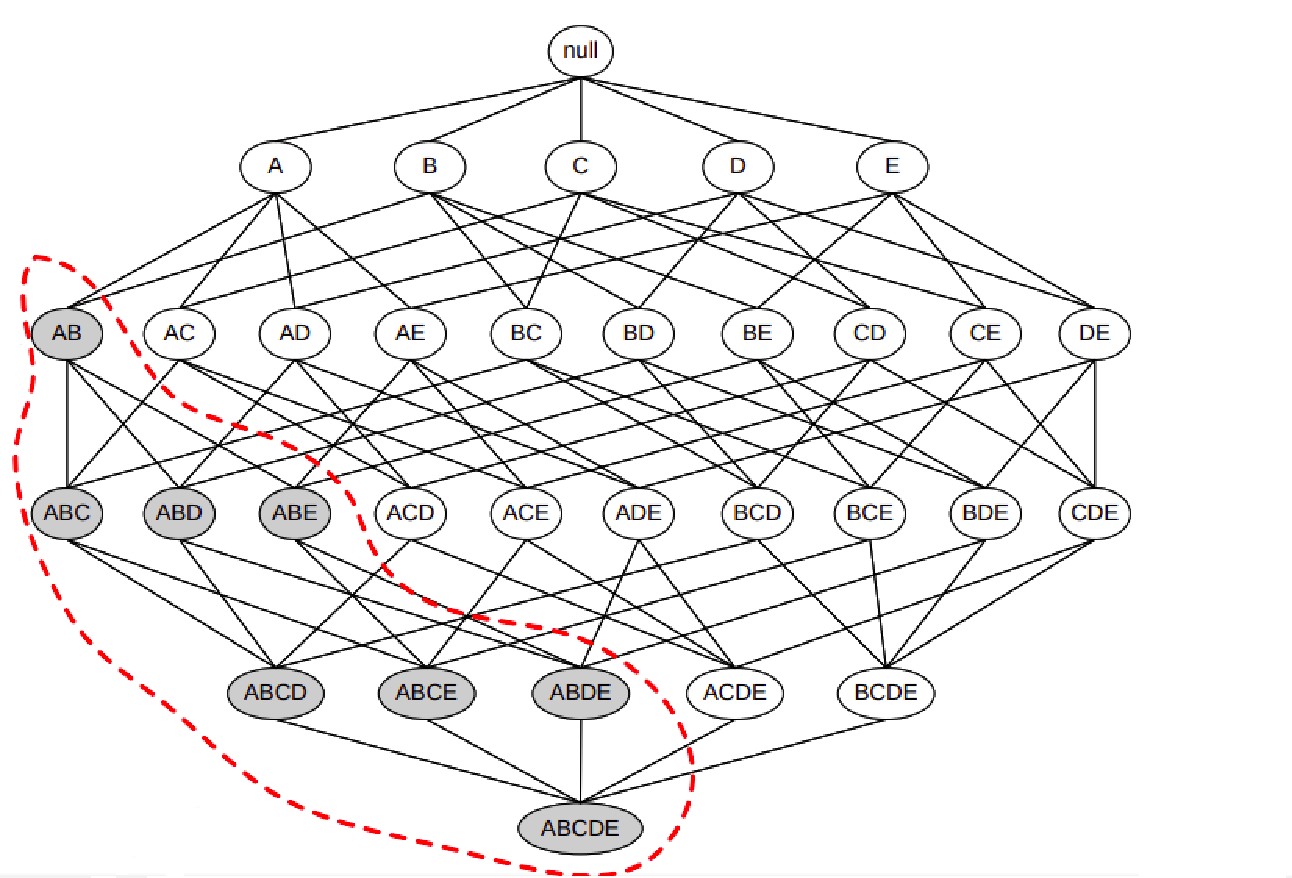
\includegraphics[scale=.8]{/sec-1/APrioriExample.pdf}
  \caption{Esempio di struttura gerarchica generata dall'algoritmo Apriori, in questo caso l'itemset \( \{ a,b \} \) non risulta frequente, di conseguenza i suoi superset sono scartati,Fonte:~\url{http://bias.csr.unibo.it/golfarelli/DataMining/MaterialeDidattico/2017/11-RegoleAssociative.pdf}}%
  \label{fig:chap-1:apriori-example}
\end{figure}

All'interno dell'insieme degli itemset validi, è possibile eseguire un'ulteriore distinzione:
si definiscono chiusi (\textit{closed}) gli itemset aventi supporto strettamente maggiore di
tutti i propri superset; al contrario un itemset non avente superset validi è definibile come
massimale (\textit{maximal}).

In molti casi Apriori è efficace nel ridurre lo spazio di ricerca di itemset validi, tuttavia
soffre di alcuni limiti: in primo luogo è molto probabile che il numero di candidati generati rimanga comunque
alto, in quanto molti di questi sono generati in un primo momento e scartati dopo il calcolo del supporto.
Prorio a quest'ultimo punto si collega un'altra problematica: la computazione del supporto richiede molte
scansioni delle transazioni e ad ogni livello devono essere verificati molti itemset.
